%% nanicolle-doc-en.tex
%% Copyright 2016--2020 Yuchang Yang < yang.yc.allium@gmail.com >
%
% This work may be distributed and/or modified under the
% conditions of the LaTeX Project Public License, either version 1.3c
% of this license or (at your option) any later version.
% The latest version of this license is in
%   http://www.latex-project.org/lppl.txt
% and version 1.3c or later is part of all distributions of LaTeX
% version 2005/12/01 or later.
%
% This work has the LPPL maintenance status `maintained'.
% 
% The Current Maintainer of this work is Yuchang Yang.
%
% This work consists of:
%   - the class file: [nanicolle.cls];
%   - the illustration files: [point.pdf, ChinaMainland.pdf, Dongguan.pdf];
%   - the manual files: [nanicolle-doc-zh.tex, nanicolle-doc-zh.pdf, 
%                        nanicolle-doc-en.tex, nanicolle-doc-en.pdf, README.md];
%   - the example files: [nanicolle-ex-zh.tex, nanicolle-ex-zh.pdf,
%                         nanicolle-ex-en.tex, nanicolle-ex-en.pdf].
%%

% arara: xelatex
% arara: xelatex

\documentclass[a4paper]{article}

\usepackage[top=32mm,bottom=32mm,textwidth=39em]{geometry}
\usepackage{marvosym}
\usepackage{metalogo}
\usepackage{rulerbox}
\usepackage{array}
	\newcolumntype{+}{>{\global\let\currentrowstyle\relax}}
	\newcolumntype{^}{>{\currentrowstyle}}
	\newcommand{\rowstyle}[1]{\gdef\currentrowstyle{#1}#1\ignorespaces}
\usepackage{enumitem}
	\setlist[description]{font=\color{mikudark}\bfseries,leftmargin=2em}
\usepackage{multicol}
	\setlength\columnsep{3em}
	\setlength\columnseprule{0.4pt}
\usepackage{adjustbox}
\usepackage{nth}
\usepackage{tikz}
\usepackage{color}
	\definecolor{mikudark}{RGB}{19, 149, 139}
\newbox\mynmy
\sbox\mynmy{%
	\smash{\raisebox{-5mm}{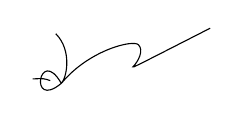
\begin{tikzpicture}[x=7mm,y=7mm]
	\draw (0,1.2)
		.. controls (0.3,0.9) and (0.2,0.4) .. (0.1,0.3)
		.. controls (-0.5,-0.2) and (-0.3,1) .. (0.1,0.3)
		.. controls (0.1005,0.299) .. (0.11,0.31)
		.. controls (0.6,0.9) and (1.4,1.1) .. (1.5,1)
		.. controls (1.6,0.9) and (1.5,0.7) .. (1.4,0.6)
		.. controls (1.39,0.58) .. (2.8,1.3);
	\draw (-0.42,0.38) .. controls (-0.22,0.39) .. (-0.1,0.35);
	\end{tikzpicture}}}}

\makeatletter
\let\url\texttt
\let\pkgname\textsf
\let\uppercase\relax
\def\zh#1{{\fontspec{SimSun}#1}}
\def\@fnsymbol#1{\ifcase#1\or*\or\Letter\fi}
\def\qtimes{\ensuremath{\times}}
\def\tab{\penalty-\@ne\kern1pt\ensuremath{\rightarrow}\kern1pt\relax}
\def\uspace{\textvisiblespace\allowbreak}
\def\@lan{\ensuremath{\langle}}
\def\@ran{\ensuremath{\rangle}}
\def\param#1{\textrm{\@lan\textit{#1}\@ran}}
\def\stopurl{\rlap{\char00}} % WHY URL IS TO GRAB EVERYTHING IT SEES?
\long\def\cmd#1{{\ttfamily\color{mikudark}#1}}
\long\def\pbox#1{\leavevmode\parbox{.86\linewidth}{\cmd{#1}}\kern-.03\linewidth}
\long\edef\[#1\]{$$\noexpand\pbox{\noexpand\raggedright#1\par}$$}
\catcode`\$=\active 
\def$#1${\cmd{#1}}
\newcount\itemcnt
	\def\clearcnt{\itemcnt\z@}
	\def\@black#1{{\color{black}\rmfamily#1}}
	\def\@theitem{\global\advance\itemcnt\@ne\@black{\romannumeral\the\itemcnt. }}
	\def\@blackperiod{\@black{. }\penalty-\tw@\@gobble}
	\def\@blackcolon{\@black{; }\penalty-\tw@}
	\def\ritem#1{\mbox{\@theitem#1}\@ifnextchar*\@blackperiod\@blackcolon}
\makeatother
	
\title{\pkgname{nanicolle} for herbarium specimen labels%
	\footnote{Github repository: \url{https://github.com/Mikumikunisiteageru/nanicolle}\stopurl.}}
\author{\zh{杨宇昌} (Yuchang \textsc{Yang})%	
	\footnote{Email address: \url{yang.yc.allium@gmail.com}\stopurl.}%
	\qquad \box\mynmy\kern-1cm}
\date{July \nth{8}, 2020\qquad ver.~2.02}
\frenchspacing 

%%%%%%%%%%%%%%%%%%%%%%%%%%%%%%%%

\begin{document}

\maketitle

\parskip=1ex\relax

Herbarium specimens are plant material well preserved as samples of plant populations. The plant material itself is insufficient to reflect all important information of the population, so it is required to prepare a fully recorded \emph{collection label} along with the material. Plant taxonomists may study a herbarium specimen and determine which species the population belongs to, and such comments are presented on \emph{identification labels} and then pasted on the specimen sheet.

\pkgname{nanicolle} is a \LaTeX\ document class for typesetting collection and identification labels for herbarium specimens, in Chinese style or in western style using English. Labels mentioned hereinafter are by default in western style, which uses a really different layout from the Chinese version (see the Chinese manual for details). Collection and identification labels can be typeset by macros $\string\collect$ and $\string\identify$ (NB: both lower case!) respectively. The output file can be printed on A4 papers (\ensuremath{297\times210} mm). 

Documents in this class can only be compiled with \XeLaTeX{}.

\pkgname{nanicolle} is distributed under the terms of \LaTeX{} Project Public License (LPPL) 1.3c\footnote{Details of the license are available on \url{http://www.latex-project.org/lppl.txt}\stopurl.}. It depends on package collection \pkgname{C\TeX{}} as well as packages including 
	\pkgname{calc}, 
	\pkgname{color}, 
	\pkgname{geometry}, 
	\pkgname{graphicx}, 
	\pkgname{listofitems}, 
	\pkgname{multicol}\footnote{Since applying \pkgname{nanicolle} document class leads to indirect use of \pkgname{multicol} package, if one wishes to employ \pkgname{nanicolle} for commercial use, he/she may be subject to moral obligation of \pkgname{multicol} (see the notice in its source file for details).}, 
	\pkgname{xstring},
etc.

\vfill\tableofcontents\vfill\null

\clearpage

%%%%%%%%%%%%%%%%%%%%%%%%%%%%%%%%

\section{Structure of documents in \pkgname{nanicolle} class}\label{usage}

A document in the \pkgname{nanicolle} class should be a plain text file with the extension \texttt{.tex}. The document generally should consist of the five following parts:
\begin{enumerate}
	\item Document class loader, i.e. $\string\documentclass[\param{option list}]\{nanicolle\}$. $\param{option}$s seperated by comma $,$ in the $\param{option list}$ control the behavior of the document. For example, $nomap$ suppresses the map on collection labels, and $autoduplicate$ repeats the collection labels according to their $\param{duplicate count}$s (vide infra). When no $\param{option}$ is specified, one can simply write $\string\documentclass\{nanicolle\}$ instead.
	\item Optional $\string\heading\{\param{heading}\}$ and $\string\subheading\{\param{subheading}\}$ in the preamble to customize content of the headings on each collection label. Both the length of $\param{heading}$ and $\param{subheading}$ should not exceed the line width. One can make a one-line heading by skipping the $\string\subheading$. If both $\string\heading$ and $\string\subheading$ are skipped, no heading will occur on the collection labels.
	\item $\string\begin\{document\}$, as the name implies.
	\item Lines starting with either $\string\collect$ or $\string\identify$ to typeset collection or identification labels respectively. Syntaxes of these macros will be declared in Section~\ref{collect} and Section~\ref{identify}. 
	\item $\string\end\{document\}$.
\end{enumerate}

%%%%%%%%%%%%%%%%%%%%%%%%%%%%%%%%

\section{The macro $\textbackslash collect$ for collection labels}\label{collect}

The syntax of the macro $\string\collect$ is
\[%
	\hangindent=2em\relax
	\string\collect
		\tab\param{record number}\tab\param{collectors}\tab\param{collecting number}%
		\tab\param{collecting date}\tab\param{family}\tab\param{vernacular name}%
		\tab\param{scientific name}\tab\param{photo number}\tab\param{duplicate count}%
		\tab\param{location}\tab\param{longitude}\tab\param{latitude}%
		\tab\param{altitude}\tab\param{habitat}\tab\param{life form}%
		\tab\param{height}\tab\param{diameter at breast height}\tab\param{note}%
\]
where $\tab$ denotes a horizontal tab (U+0009, the character that the tab key inputs). Each $\string\collect$ macro followed by its parameters must exclusively occupy a single line without comment sign, and the line should begin immediately with the macro. 
Parameters can be left empty (some cannot), but even so the tabs seperating them should never be omitted. 
The requirements of each parameter of $\string\collect$ are listed as follows. 

\begin{enumerate}
	\item $\param{record number}$: Only for the convenience of data organizing, not printed on collection label.
	\item $\param{collectors}$: Names of the persons or the team who collected the specimen. When there were more than one collectors, all their names should be listed here. When a team was involved, it is strongly suggested to list its members' names in parentheses after the team name. $\param{collectors}$ \textsl{cannot} be empty. 
	\item $\param{collecting number}$: Serial number indexing the specimen collection of the first component of $\param{collectors}$. Traditionally it is suggested to apply sequences of increasing integers starting from 1 to $\param{collecting number}$.
	\item $\param{collecting date}$: Date when the specimen was collected, better expressed in arabic numerals following the formula $\param{year}.\param{month}.\param{date}$. Parameter $\param{collecting date}$ \textsl{cannot} be empty. 
	\item $\param{family}$: Preliminary scientific name (in Latin) of the family.
	\item $\param{vernacular name}$: Preliminary vernacular name of the species, in local language. Not printed on collection label.
	\item $\param{scientific name}$: Preliminary scientific name (in Latin) of the species, better with no author citation especially when uncertain. Unless empty, $\param{scientific name}$ follows the fomula $\param{generic part}\param{specific part}\param{infraspecific part}$. \par
		In the formula above, there are two possible patterns for the $\param{generic part}$:
		\[\clearcnt
			\ritem{\param{genus name}}%
			\ritem{\qtimes\param{genus name}}*\]
		$\param{specific part}$ has nine possible patterns:
		\[\clearcnt
			\ritem{\uspace sp.}%
			\ritem{\uspace sp.\uspace nov.}%
			\ritem{\uspace\param{species epithet}}%
			\ritem{\uspace\qtimes\param{species epithet}}%
			\ritem{\uspace aff.\uspace\param{species epithet}}%
			\ritem{\uspace aff.\uspace\qtimes\param{species epithet}}%
			\ritem{\uspace cf.\uspace\param{species epithet}}%
			\ritem{\uspace cf.\uspace\qtimes\param{species epithet}}%
			\ritem{\uspace '\param{cultispecies name}'}*\]
		where $\uspace$ denotes a normal space (U+0020). 
		$\param{infraspecific part}$ can be not empty when and only when $\param{specific part}$ fits its pattern iii or iv, at this time having four possible patterns:
		\[\clearcnt
			\ritem{\uspace subsp.\uspace\param{subspecific epithet}}%
			\ritem{\uspace var.\uspace\param{varietal epithet}}%
			\ritem{\uspace f.\uspace\param{form epithet}}%
			\ritem{\uspace '\param{cultivar name}'}*\]
    Control sequences like $\string\textit$ manually designating font style are unavailable in $\param{scientific name}$.
	\item $\param{photo number}$: Only for the convenience of data organizing, not printed on collection label.
	\item $\param{duplicate count}$: Count of specimen duplicates with the same $\param{collecting number}$, expressed in arabic numerals; not printed on collection label. When $autoduplicate$ is loaded as an $\param{option}$ of the document class, each $\string\collect$ macro automatically makes $\param{duplicate count}$ duplicate collection labels.
	\item $\param{location}$: Location where the specimen was collected, expressed in natural way, providing as much detailed information as possible, including country, province, city, town, etc., and the specific locality (probably with respect to some landmarks), so that other researchers can locate the population. $\param{location}$ \textsl{cannot} be empty.
	\item $\param{longitude}$: Longitude value of the $\param{location}$, a decimal floating number in degree (without unit), positive for east, negative for west. Sexagesimal expression (in degree, minute, and second) are not acceptable.
	\item $\param{latitude}$: Latitude value of the $\param{location}$, a decimal floating number in degree (without unit), positive for north, negative for south. Sexagesimal expression (in degree, minute, and second) are not acceptable.
	\item $\param{altitude}$: Altitude value of the $\param{location}$, in meter (without unit), positive or possibly negative.
	\item $\param{habitat}$: Living habitat of the population in the wild, e.g. $slopes$, $forest margins$, $streamsides$; or $cultivated$ for those in garden or arboretum.
	\item $\param{life form}$: Life form of typical individuals in the population, e.g. $tree$, $shrub$, $vine$.
	\item $\param{height}$: Height of typical individuals in the population, in meter (without unit). 
	\item $\param{diameter at breast height}$: Diameter at breast height (DBH) of typical individuals in the population, in centimeter (without unit), only applying to trees or large shrubs.
	\item $\param{note}$: Other valuable information that is no longer observable on herbarium specimens, in aspects of morphology (e.g. color \& smell of different parts, texture of the bark), ecology (e.g. richness, pollinator species), or ethnobotany (e.g. local usages). Different from other parameters of $\string\collect$, $\param{note}$ is a complete sentence (unless empty), so that the leading letter of the first word should be capitalized, and a punctuation (usually period) is required at the end.
\end{enumerate}

\def\degree{\kern0.1ex\ensuremath{^\circ}}
By default, when preparing a collection label, \pkgname{nanicolle} typesets a map below the main body of the label, illustrating the position of the coordinates, given that the $\param{longitude}$ lies between 73\degree E and 136\degree E, and the $\param{latitude}$ lies between 17\degree N and 54\degree N. One can load a $nomap$ $\param{option}$ into the document class (Section~\ref{usage}) to suppress the typesetting of maps. It is also possible to redefine the geographic range of the maps. 

%%%%%%%%%%%%%%%%%%%%%%%%%%%%%%%%

\section{The macro $\textbackslash identify$ for identification labels}\label{identify}

The syntax of the macro $\string\identify$ is
\[%
	\hangindent=2em\relax
	\string\identify
		\tab\param{record number}\tab\param{scientific name}\tab\param{vernacular name}%
		\tab\param{identifier}\tab\param{identifier code}%
		\tab\param{identifying date}\tab\param{comment}%
\]
Just as $\string\collect$, each $\string\identify$ macro with its parameters must exclusively occupy a single line. 
Parameters can be left empty unless specialized, but the tabs seperating them cannot be omitted. 
The requirements of each parameter of $\string\identify$ are listed as follows. 

\begin{enumerate}
	\item $\param{record number}$: Only for the convenience of data organizing, not printed on identification label.
	\item $\param{scientific name}$: Scientific name with author citation of the species that the identification yielded, following the formula $\param{generic part}\param{specific part}\param{infraspecific part}\uspace\param{author citation}$. As that of $\string\collect$, macros for manually manipulating font style are unavailable here either. $\param{scientific name}$ \textsl{cannot} be empty.
	\item $\param{vernacular name}$: Common name associated with $\param{scientific name}$ of the species.
	\item $\param{identifier}$: Full name of the identifier.
	\item $\param{identifier code}$: Standard form (taxonomic) of the name of the identifier. $\param{identifier}$ and $\param{identifier code}$ \textsl{cannot} be both empty, while it is suggested to leave either of them empty in a record. 
	\item $\param{identifying date}$: Date when the specimen was identified, following the same restriction as $\param{collecting date}$ for $\string\collect$. $\param{identifying date}$ \textsl{cannot} be empty.
	\item $\param{comment}$: Comment about the identification worth mention. Different from other parameters of $\string\identify$, $\param{comment}$ is a complete sentence (unless empty), so that the leading letter of the first word should be capitalized, and a punctuation (usually period) is required at the end.
\end{enumerate}

The $\string\identify$ macro has no $\param{duplication count}$ parameter, so identification label will not be automatically repeated. When repeating is wanted, one has to repeat the lines with $\string\identify$ manually.

%%%%%%%%%%%%%%%%%%%%%%%%%%%%%%%%

\section{Other issues}

\subsection{Store original data in a spreadsheet software}

Using tabs $\tab$ as delimiters between parameters is not the convention of \LaTeX{}. This special rule for delimiters was designed to make \pkgname{nanicolle} able to read the plain text lines from a spreadsheet software\footnote{Microsoft Office Excel is an instance of spreadsheet software.}. When some rows of cells are pasted from a spreadsheet software to plain text environment, it is automatically converted to TSV (Tab-Separated Values) format --- rows/lines are separated by end-of-line character(s), and cells within a row/line are separated by tab. This mechanism allows users to establish a database for collection or identification records in a spreadsheet software (as Table~\ref{table}). When one wants to print labels according to certain records, he/she can simply copy the involved rows from the database, paste them in a \LaTeX{} source file, and then call \pkgname{nanicolle} to deal with them. Databases can also contain extra information after the parameters required, which will be ignored by $\string\collect$ or $\string\identify$ and will not affect the output. 

\begin{table}[htbp]
	\centering
	\begin{tabular}{|+c|*{4}{^c|}}
		\hline
		\rowstyle{\bfseries} macro & record number & collectors & collecting number & \ensuremath{\cdots} \\\hline
		\string\collect & 1 & Foo, Bar & 3141 & \ensuremath{\cdots} \\\hline
		\string\collect & 2 & Foo, Bar & 3142 & \ensuremath{\cdots} \\\hline
		\string\collect & 3 & Foo, Bar & 3143 & \ensuremath{\cdots} \\\hline
	\end{tabular}
	\caption{A sample of database for collection records in a spreadsheet database}\label{table}
\end{table}

\subsection{Set the printer correctly}

Before the PDF file from \pkgname{nanicolle} is sent to a printer, it is necessary to do some settings. When printing an A4-sized PDF file on to an A4-sized paper with a home printer, the file is usually shrunk a little bit smaller to fit into the printable range. If so, since \pkgname{nanicolle} uses a four-column landscape layout, the outer columns would be some broader than the inner ones. To avoid unbalance, one can select to print ``at actual size'', ``at absolute size'', or make the scale ``100\%''.

%%%%%%%%%%%%%%%%%%%%%%%%%%%%%%%%

\section{Change history}

\pkgname{nanicolle} was originally designed for making Chinese collection labels and identification labels, with its first version completed on 2016/8/3 (ver. 1.01). Later on 2017/10/22 (ver. 1.07), the typesetting of western style collection labels was carried out for an international plant expedition, and that was the first version with maps. The macro for collection labels in western style had been temporarily hidden since 2019.4.28 (ver. 2.00), until rewritten and republished on 2020.7.8 (ver. 2.02). 
For more details, please refer to the Chinese manual \texttt{nanicolle-zh.PDF}. 

%%%%%%%%%%%%%%%%%%%%%%%%%%%%%%%%

\section{A full example using \pkgname{nanicolle}}

The following is a full example file using document class \pkgname{nanicolle}. It can be found as \texttt{nanicolle-ex-en.tex} in the package. To display it more clearly, the $\uspace$ denotion for space is no longer used in this example. Actual lines correspond with line numbers in the left. An actual line may be so long that it is wrapped here, just as in text editors, but remember, these wrapped parts in fact belong to a single line, as there is no end-of-line character in between. 

\begingroup
\catcode`\^^I\active\let^^I\tab
\[%
\clearcnt
\def\zh#1{{\fontspec{FangSong}#1}}
\everypar={\hangindent=2em\relax\advance\itemcnt1\relax%
\leavevmode\llap{\number\itemcnt\quad}}
\string\documentclass[autoduplicate]\string{nanicolle\string}\par
\string\begin\string{document\string}\par
\string\collect	1997	Yuchang Yang (\zh{杨宇昌})	5731	2018.5.8	Caprifoliaceae	\zh{苦糖果}	Lonicera fragrantissima subsp. standishii	7609	1	between Dongjiamen Village (\zh{董家门村}) and Dongnao (\zh{洞垴}), Guantao Town (\zh{管陶乡}), Wu'an City (\zh{武安市}), Hebei Province (\zh{河北省}), China	113.759512	36.951612	1356.0	meadow thickets on slopes	shrub	3		Ripe fruit orange-red, tasting sweet with minimal bitter.\par
\string\collect	1545	Sino-Nepal Joint Plant Expedition (Haining Qin, Prabin Bhandari, Tirtha Raj Pandey, Bijay Raj Subedee, Yuchang Yang, Shuren Zhang)	601	2017.9.18	Fagaceae		Quercus glauca	-	2	Talkot, Bajhang District, Nepal			1700	forests	tree	10	15	Fruiting. Associated with \string\textit\string{Rhododendron arboreum\string} and \string\textit\string{Lyonia ovalifolia\string}.\par
\string\identify	392	Allium atrosanguineum var. tibeticum (Regel) G. H. Zhu \string& Turland	\zh{藏葱} (Z\string\`ang C\string\=ong)	Yuchang Yang		2018.10.7	\par
\string\identify	176	Acer davidii subsp. grosseri (Pax) P. C. de Jong		Yuchang Yang		2018.4.19	\par
\string\identify	230	Erysimum \qtimes cheiri (L.) Crantz		Yuchang Yang		2018.5.17	\par
\string\identify	590	Koenigia alpina (All.) T. M. Schust. \string& Reveal		Yuchang Yang		2019.4.13	\par
\string\end\string{document\string}\par
\]
\endgroup

Locate to the path of the example file in a command line window, then type and execute \texttt{xelatex nanicolle-ex-en}. After the compilation, the output PDF file (see Figure~\ref{example}) \texttt{nanicolle-ex-en.PDF} can be found in the same path.

\begin{figure}[htbp]
	\centering
	\fboxsep=-.2pt\relax
	\hbox{}\hidewidth\rulerbox{\vbox{\kern-.2pt\hbox{\kern-.2pt\fbox{\includegraphics*[bb=0cm 0cm 14.85cm 21cm]{nanicolle-ex-en.pdf}}\kern-.2pt}\kern-.2pt}}\hidewidth\hbox{}\par
	\caption{Left two columns in the sample PDF file \texttt{nanicolle-ex-en.pdf}}\label{example}
\end{figure}

\end{document}
